\documentclass[a4paper,11pt,final,fleqn]{article}

% Import des packages
\usepackage{../fsab}
\usepackage[french]{babel}
\usepackage{fancybox}
\usepackage{shortvrb}
\usepackage{adjustbox}
\usepackage{url}
\usepackage{fourier}
\usepackage{hyperref}


% Style des listings
\lstset{rulesepcolor=\color{black},framesep=2pt,frame=shadowbox,numberstyle=\tiny}
\setlength{\shadowsize}{2pt}

\newcolumntype{C}{>{\centering\arraybackslash}p}

\lstnewenvironment{stdout}{\lstset{numbers=none,language={},frame=single,backgroundcolor=\color[gray]{0.9},framerule=2mm,rulecolor=\color[gray]{0.9},xleftmargin=3mm,xrightmargin=3mm,belowskip=2mm}}{}

% Informations sur le document
\def\doctitle{Projet - Eternity II}
\def\docsigle{INF6102}
\def\docversion{Hiver 2022}
\def\docdest{Étudiants}
\def\docauthor{{\tiny QC, GR}}


\begin{document}

\printtitle

% - - - - - - - - - - - - - - - - - - - - - - - - - - - - - - - - - - - - - - - - - - - - - - - - - - - - - - - - - - - - - -

\textbf{Remise le $17/04/2022$ (avant minuit) sur Moodle pour tous les groupes.}

\section*{Consignes}

\begin{itemize}
      \item[$\bullet$]  Le projet doit être fait par groupe de 2 au maximum. Il est
            fortement recommandé d'être 2.
      \item[$\bullet$] Lors de votre soumission, donnez votre rapport
            au format \textbf{PDF} (matricule1\_matricule2\_Projet.pdf)
      \item[$\bullet$] Lors de votre soumission, votre code \texttt{xx.py} et ses dépendances doivent être au format \textbf{ZIP} (matricule1\_matricule2\_Projet.zip).
      \item[$\bullet$] Indiquez vos noms et matricules dans le fichier PDF et en commentaires en haut du fichier de code soumis.
      \item[$\bullet$] Toutes les consignes générales du cours (interdiction de
            plagiat, etc.) s'appliquent pour ce devoir.
      \item[$\bullet$] Il est permis (et encouragé) de discuter de vos pistes de solution avec les autres groupes. Par contre, il est formellement interdit de reprendre le code d'un autre groupe ou de copier un code déjà existant (StackOverflow ou autre). Tout cas de plagiat sera sanctionné de la note minimale pour le projet.
\end{itemize}


\section*{Enoncé du projet}

\texttt{Eternity II} est un célèbre puzzle\footnote{\url{https://en.wikipedia.org/wiki/Eternity_II_puzzle}} demandant de remplir un plateau de taille $16\times 16$ avec 256 cases. Chaque case est divisée en 4 zones contenant une couleur différente pour chaque bord. 
Une case ne peut être adjacente qu'à une autre case ayant la même couleur au bord adjacent. Un exemple simplifié avec 16 cases pour un plateau $4\times 4$ vous est présenté ci-dessous.

\begin{figure}[!ht]
\centering
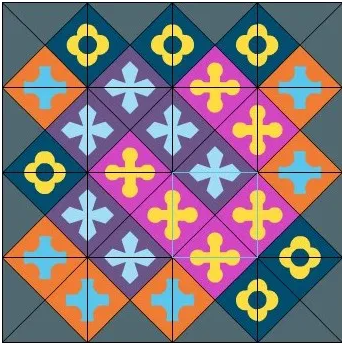
\includegraphics[width=0.25\textwidth]{img/eternity}
\end{figure}


La renommée de ce jeu vient du fait que son créateur, \textit{Christopher Monckton}, confiant sur sa difficulté a promis une somme de 2 millions de dollars à 
la première personne trouvant une solution. Le défi a été lancé à la sortie du jeu (2007), et avait pour échéance la date du 31 décembre 2010. Personne 
n'a réussi ce défi. La meilleure solution trouvée avant l'échéance avait 467 connexions correctes, sur les 480. A l'heure actuelle, personne n'a encore 
réussi à résoudre ce puzzle. 

Ce projet vous demandera de développer un algorithme innovant basé sur les heuristiques, la recherche locale, et les métaheuristiques pour résoudre au mieux 
ce problème. Évidemment, résoudre le problème de base ne sera pas requis pour obtenir la totalité des points (des instances plus simples seront proposées), 
mais vous permettra de pousser à l'extrême les capacités de vos algorithmes et à - \textit{qui sait} - améliorer l'état de l'art pour ce puzzle. 
De plus, le meilleur résultat apparaîtra dans le \textit{Hall of fame} du cours pour les prochaines années. :-)

De manière plus formelle, le problème est le suivant. Vous avez un certain nombre de tuiles à votre disposition. Celles-ci sont carrées. 
Elle sont également divisées en 4 triangles. Ces triangles sont colorés d'un certain motif. Le jeu consiste à placer toutes les tuiles sur le plateau de 
telle sorte que chaque paire de tuile voisine aie le même motif sur leur triangle adjacent. Une rotation peut également être effectuée sur chaque tuile. 
Une couleur spéciale (gris dans notre exemple) correspond au bord du plateau.

Les fichiers contenant les instances du problème sont organisés en $n^2+1$ lignes.
La première ligne contient un entier: la dimension $n$ du plateau.
Chacune des $n^2$ lignes suivante correspond à une tuile. La tuile est composée de 4 entiers. Chacun d'entre eux correspond à un identifiant de motif. 
Le premier motif est celui du nord, le second, celui du sud, puis celui de l'ouest et finalement celui de l'est.

\begin{lstlisting}
  n
  c_1N c_1S C_1W C_1E
  c_2N c_2S C_2W C_2E
  ...
  c_nN c_nS C_nW C_nE
\end{lstlisting}

Le format d'une solution attendue comporte $n^2+2$ lignes. 
La première ligne contient un entier qui donne le nombre de conflits de la solution, la seconde donne la dimension $n$ de l'instance, 
les autres $n^2$ lignes donnent les tuiles dans un ordre qui commence en bas à gauche, liste les tuiles de la première ligne, puis la deuxième 
(celle au dessus de la première), etc. jusqu'à la dernière ligne pour finir sur la dernière tuile en haut à droite. Le code de la tuile est dans le 
même ordre que pour le fichier d'entrée (nord, sud, ouest, est), tenant compte de la rotation que vous appliquer à la tuile.
\begin{lstlisting}
  totValue
  n
  C_1N C_1S C_1W C_1E
  C_2N C_2S C_2W C_2E
  ...
  C_nN C_nS C_nW C_nE
\end{lstlisting}

A titre d'exemple, l'instance suivante est un plateau de $2 \times 2$, avec 4 cases.

\begin{lstlisting}
2
1 0 0 2
3 0 0 1
4 0 0 3
2 0 0 4
\end{lstlisting}

Une possible solution au problème est la configuration suivante, qui engendre 6 conflits. 
\begin{lstlisting}
6
2
0 4 3 0 
1 0 0 2 
0 1 0 3 
0 2 4 0 
\end{lstlisting}

Visuellement, cela donne ceci:

\begin{figure}[!ht]
\centering
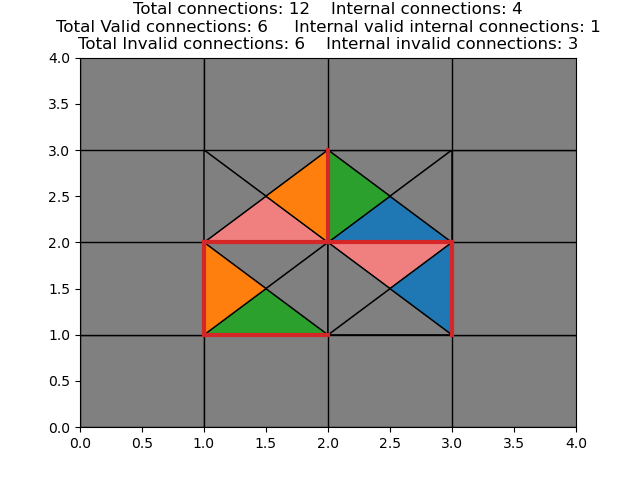
\includegraphics[scale=0.4]{img/eternity_ex}
\end{figure}

\section*{Implémentation}

Vous avez à votre disposition un projet python.
Plusieurs fichiers vous sont fournis:

\begin{itemize}
\item \texttt{eternity\_puzzle.py}:  contient toute la logique du jeu Eternity II et des fonctions utiles pour construire une solution.  Vous êtes
libre de changer les fonctions de ce fichier si vous voulez rendre certaines opérations efficaces. 

\textbf{\danger Dans ce cas là, il est de votre responsabilité de vous assurer que vos modifications sont correctes vis-à-vis des règles du jeu.}
\item \texttt{main.py}: permet d'exécuter un de vos algorithmes sur une instance donnée. Vous obtiendriez en retour un fichier .txt reprenant
votre solution, ainsi qu'une image .png la représentant graphiquement.
\item \texttt{solver\_random.py}: implémentation d'un solveur résolvant le problème de manière aléatoire. Ce solveur effectue 1 million de constructions
aléatoires et prend la meilleure configuration trouvée.
 \item \texttt{solver\_heuristic.py}: implémentation que vous devez fournir (phase 1 du projet) 
  \item \texttt{solver\_local\_search.py}: implémentation que vous devez fournir (phase 2 du projet) 
   \item \texttt{solver\_advanced.py}: implémentation que vous devez fournir (phase 3 du projet). 
   Ce solveur constitue le coeur du projet et correspond à votre agent le plus efficace.
\end{itemize}

Vous êtes également libres de rajouter d'autres fichiers au besoin. De plus, 8 instances sont mises à votre disposition:

\begin{itemize}
\item \texttt{eternity\_trivial\_A.txt}: plateau $2 \times 2$ pour tester votre implémentation (ne rapporte aucun point).
\item \texttt{eternity\_trivial\_B.txt}: plateau $3 \times 3$ pour tester  votre implémentation (ne rapporte aucun point).
\item \texttt{eternity\_A.txt}: plateau $4 \times 4$, utilisé pour la évaluer la qualité de votre solveur.
\item \texttt{eternity\_B.txt}: plateau $7 \times 7$, utilisé pour la évaluer la qualité de votre solveur.
\item \texttt{eternity\_C.txt}: plateau $8 \times 8$, utilisé pour la évaluer la qualité de votre solveur.
\item \texttt{eternity\_D.txt}: plateau $9 \times 9$, utilisé pour la évaluer la qualité de votre solveur.
\item \texttt{eternity\_E.txt}: plateau $10 \times 10$, utilisé pour la évaluer la qualité de votre solveur.
\item \texttt{eternity\_complet.txt}: jeu de base ($16 \times 16$), donnant un bonus pour la meilleure équipe.
\end{itemize}

Pour vérifier que tout fonctionne bien, vous pouvez exécuter l'agent aléatoire comme suit.

\begin{lstlisting}
python3 main.py --agent=random --infile=instances/eternity_A.txt 
\end{lstlisting}

Un fichier \texttt{solution.txt} et une image \texttt{visualization.png} seront générés.

\section*{Production à réaliser}

Le projet est constitué de 4 phases, détaillés ci dessous.

\paragraph{Phase 1: solveur heuristique} Vous devez compléter le fichier \texttt{solver\_heuristic.py} avec un algorithme heuristique. 
C'est à dire que votre algorithme va construire une solution complète étape par étape (pièce par pièce) suivant une heuristique que vous devez définir.
Il n'est pas attendu que cette méthode donne d'excellents résultats, mais elle vous permettra de vous familiariser avec le projet et le code mis à disposition. De plus, les heuristiques que vous utilisez pourront être utilisées dans les implémentations de vos autres algorithmes. 
Il est donc intéressant de bien réfléchir à cette tâche. L'heuristique que vous aurez considérée devra être détaillée succinctement dans le rapport du projet. L'agent peut ensuite être exécuté comme suit.

\begin{lstlisting}
python3 main.py --agent=heuristic --infile=instances/eternity_A.txt 
\end{lstlisting}

\textit{Début suggéré}: dès l'annonce du projet.

 
\paragraph{Phase 2: solveur de recherche locale} Vous devez compléter le fichier \texttt{solver\_local\_search.py} avec un algorithme de recherche locale. C'est à dire que votre algorithme va partir d'une solution complète et l'améliorer petit à petit via des mouvements locaux. 
Réfléchissez bien à la définition de votre espace de recherche, de votre voisinage, fonction de sélection et d'évaluation.
Vous devez également rajouter un mécanisme de \textit{restarts} et/ou du \textit{simulated annealing} pour permettre à votre recherche de s'échapper des minima locaux.  Il n'est pas attendu que cette méthode donne d'excellents résultats, mais elle devrait être bien meilleure qu'une 
heuristique simple. Le modèle de recherche locale que vous aurez considéré devra être détaillé succinctement dans le rapport du projet.
L'agent peut ensuite être exécuté comme suit.

\begin{lstlisting}
python3 main.py --agent=local_search --infile=instances/eternity_A.txt 
\end{lstlisting}

\textit{Début suggéré}: dès que le module \textit{recherche locale} a été vu.


\paragraph{Phase 3: solveur avancé}  Vous devez compléter le fichier \texttt{solver\_advanced.py} avec votre méthode finale de résolution. 
Cet agent constitue la plus grande partie du projet et est celui vous apportant le plus de points dans ce projet. Vous êtes entièrement libre d'utiliser tous les mécanismes que vous souhaitez pour implémenter cet agent. On vous conseille néanmoins d'expérimenter avec les méta-heuristiques vues au cours et d'y ajouter vos propres idées.  Également, les métaheuristiques ne sont pas incompatibles entre elles, vous pouvez également imaginer des approches hybrides. 
Cet agent devra être expliqué en détail dans le rapport du projet. En particulier, veillez à bien détailler vos différents choix de conceptions.
Finalement, vous pouvez également vous inspirer d'approches présentes dans la littérature scientifique. Dans ce cas, veillez à bien mentionner vos références et inspirations dans le rapport.

\begin{lstlisting}
python3 main.py --agent=advanced --infile=instances/eternity_A.txt 
\end{lstlisting}

\textit{Début suggéré}: dès que les première méta-heuristiques ont été vues.


\paragraph{Phase 4: analyse des performances} A l'issue des 3 phases précédentes, vous avez à disposition 4 solveurs (aléatoire, heuristique simple, recherche locale, algorithme avancé). Il vous est maintenant demandé de réaliser des analyses pertinentes sur l'efficacité de ces agents sur les 8 instances fournies. A titre d'exemple, il est intéressant de comparer le temps d'exécution des différentes méthodes, la qualité de la solution trouvée, comment la meilleure solution évolue en fonction du temps d'exécution, etc. Proposez également une analyse qualitative de votre agent: ses forces, ses faiblesses, ses limitations,  la taille du voisinage, complexité des fonctions utilisées, etc.

\textit{Début suggéré}: dès que le module sur l'évaluation des solveurs a été vu.

\section*{Critères d'évaluation}

L'évaluation portera sur la qualité du rapport et du code fournis, ainsi que sur les performances de votre solveur sur les différentes instances.
Concrètement, la répartition des points (sur 20) est la suivante:

\begin{itemize}
\item 1 point sur 20 est attribué à l'implémentation de votre solveur heuristique. 
\item 2 points sur 20 sont attribués à l'implémentation de votre solveur de recherche locale.
\item 7 points sur 20 sont attribués à l'implémentation de votre solveur avancé. 
Les instances \textit{A}, \textit{B}, et \textit{C} rapportent 1 point si une solution faisable est obtenue, et 0 sinon. Les instances  \textit{D}, \textit{E} rapportent 2 points si une solution faisable est obtenue et diminue progressivement jusqu'à 0 en fonction de la qualité de la solution. 
Si aucun groupe ne trouve une solution faisable pour ces instances, la solution du meilleur groupe est prise comme référence des 2 points.
Le temps d'exécution autorisé pour chaque instance est de 1 heure\footnote{Vous pouvez supposer que l'ordinateur qu'on utilisera pour exécuter vos algorithmes aura une performance de calcul supérieur au vôtre (calcul parallèle non inclus).}.
\item 10 points sur 20 sont attribués pour le rapport.  Pour ce dernier, les critères sont la qualité générale, la qualité des explications, le détail des choix de conception, la pertinence et la rigueur du protocole expérimental.
\item 2 points bonus seront attribués au groupe ayant le meilleur résultat pour l'instance complète. Aucune restriction sur le temps d'exécution n'est imposée.
\end{itemize}

\textbf{\danger Il est attendu que vos algorithmes retournent une solution et un coût correct. Par exemple, il est interdit d'ajouter de nouvelles pièces, de modifier artificiellement le nombre de conflits ou autre. Un algorithme retournant une solution non cohérente est susceptible de recevoir aucun point.}

\section*{Conseils}

Voici quelques conseils pour mener le projet à bien:

\begin{enumerate}
\item Le projet a été conçu pour que le travail puisse bien être réparti tout au long de la session. Profitez-en !
La première phase peut être commencée dès maintenant.
\item Tirez le meilleur parti des séances de laboratoire encadrées afin de demander des conseils.
\item Inspirez vous des techniques vues au cours, et ajoutez-y vos propres idées.
\item Tenez compte du fait que l'exécution de vos algorithmes peut demander un temps considérable.
Dès lors, ne vous prenez pas à la dernière minute pour réaliser vos expériences.
\item Le temps d'exécution est volontairement long pour refléter des expériences réelles que vous effectuerez plus tard dans des applications industrielles. Organisez au mieux votre temps de développement/évaluation. Par exemple, une bonne pratique est d'évaluer votre algorithme la nuit sur un serveur lorsque vous ne travaillez pas.
\end{enumerate}


\section*{Remise}
Vous devez remettre une archive zip contenant:
\begin{itemize}
\item Votre code au complet.
\item les solutions obtenues sur chacune des instances non-triviales à votre disposition (les fichiers solution doivent être nommés "solutionX" avec X la lettre correspondant à l'instance)
\item un rapport de 5 pages au maximum (page de garde non comprise) reprenant les informations demandées plus haut.
\end{itemize}

Bon travail, bonne chance, et surtout, amusez vous !

\section*{Hall of fame}
Récapitulatifs des meilleures solutions obtenue jusqu'à présent pour le problème complet.

\begin{enumerate}
\item Score de 404/480 (H21 - Maxime F. et Daniel D.)
\end{enumerate}

\begin{figure}[!ht]
\centering
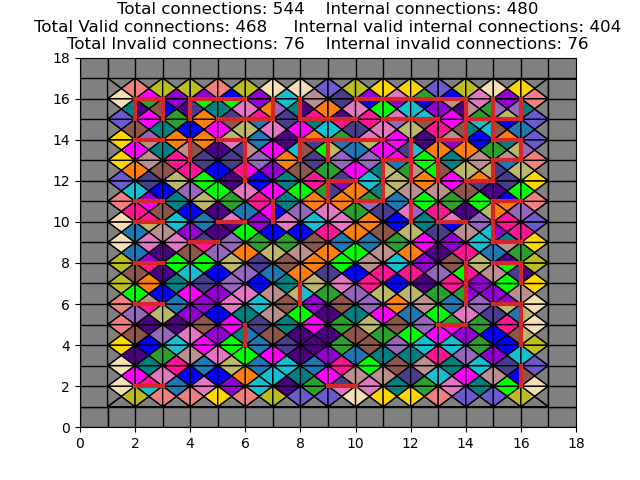
\includegraphics[width=0.75\textwidth]{img/best-sol-so-far}
\end{figure}

\end{document}

